\documentclass[11pt,a4paper]{article}

% ---------- Sprache & Encoding ----------
\usepackage[utf8]{inputenc}
\usepackage[T1]{fontenc}
\usepackage{lmodern}

% ---------- Layout ----------
\usepackage[a4paper,margin=2.3cm]{geometry}
\usepackage{enumitem}
\usepackage{booktabs}
\usepackage{array}
\usepackage{tabularx}
\usepackage{graphicx}
\usepackage{amsmath,amssymb}
\usepackage{xcolor}
\usepackage{tcolorbox}
\tcbuselibrary{skins,breakable}
\usepackage{fancyhdr}
\usepackage[hidelinks]{hyperref}
\usepackage{titlesec}
\usepackage{tikz}
\usetikzlibrary{arrows.meta}
\usepackage{comment}

% ---------- Farben ----------
\definecolor{kfrblue}{HTML}{1F5C99}
\definecolor{warnorange}{HTML}{B45309}
\definecolor{warnbg}{HTML}{FFF3E0}
\definecolor{tipbg}{HTML}{EAF3EA}
\definecolor{tipgreen}{HTML}{2E7D32}

% ---------- Überschriften ----------
\titleformat{\section}{\large\bfseries\color{kfrblue}}{\thesection}{0.6em}{}
\titleformat{\subsection}{\normalsize\bfseries\color{kfrblue}}{\thesubsection}{0.6em}{}

% ---------- Kopf-/Fusszeile ----------
\pagestyle{fancy}
\fancyhf{}
\renewcommand{\headrulewidth}{0.4pt}
\fancyhead[L]{\small Physik 5.\,Klasse, Praktikum 09}
\fancyhead[R]{\small Reflexion und Brechung}
\fancyfoot[C]{\small\thepage}

% ---------- Boxen ----------
\newtcolorbox{achtungbox}[1][]{%
  colback=warnbg, colframe=warnorange, coltitle=white, colbacktitle=warnorange,
  boxrule=0.8pt, arc=2pt,
  left=6pt, right=6pt, top=4pt, bottom=4pt, breakable,
  title={\textbf{Achtung: darauf kommt es an}#1},
  fonttitle=\small, fontupper=\small
}
\newtcolorbox{tippbox}[1][]{%
  colback=tipbg, colframe=tipgreen, coltitle=white, colbacktitle=tipgreen,
  boxrule=0.8pt, arc=2pt,
  left=6pt, right=6pt, top=4pt, bottom=4pt, breakable,
  title={\textbf{Merke}#1},
  fonttitle=\small, fontupper=\small
}
\newtcolorbox{aufgabebox}[1][]{%
  colback=gray!6, colframe=kfrblue, coltitle=white, colbacktitle=kfrblue,
  boxrule=0.8pt, arc=2pt,
  left=6pt, right=6pt, top=4pt, bottom=4pt, breakable,
  title={\textbf{Aufgabe}#1},
  fonttitle=\small, fontupper=\small
}
\newtcolorbox{loesungbox}[1][]{%
  colback=tipbg, colframe=tipgreen, coltitle=white, colbacktitle=tipgreen,
  boxrule=0.8pt, arc=2pt,
  left=6pt, right=6pt, top=4pt, bottom=4pt, breakable,
  title={\textbf{Lösung}#1},
  fonttitle=\small, fontupper=\small
}

% ---------- Lösungen: Solutions-Toggle ----------
\newcommand{\printanswers}{\includecomment{solution}}
\newcommand{\noprintanswers}{\excludecomment{solution}}
\noprintanswers   % Schülerversion (Standard)
% \printanswers   % Lösungsversion: diese Zeile aktivieren, obige auskommentieren

\setlist[itemize]{leftmargin=1.4em, itemsep=2pt, topsep=3pt}
\setlist[enumerate]{leftmargin=1.6em, itemsep=2pt, topsep=3pt}

% ---------- einfache Einheiten-Makros (kein siunitx nötig) ----------
\newcommand{\celsius}{\ensuremath{^{\circ}\mathrm{C}}}
\newcommand{\SI}[2]{#1\,#2}

% ---------- Platz für freie Antworten/Zeichnungen (leer, ohne Linien/Karos) ----------
\newcommand{\zeichenraum}[1][4.5cm]{%
  \par\vspace{4pt}\noindent
  \fbox{\begin{minipage}[t][#1][t]{\dimexpr\linewidth-2\fboxsep-2\fboxrule}\ \end{minipage}}
  \vspace{4pt}
}

\begin{document}
\thispagestyle{empty}

% ---------- Titelblock ----------
\begin{center}
  {\color{kfrblue}\Large\bfseries Praktikum 09: Reflexion und Brechung}\\[2pt]
  {\normalsize Kantonsschule Freudenberg, Physik 5.\ Klasse}
\end{center}

\vspace{4pt}
\noindent
\begin{tabularx}{\linewidth}{@{}X X@{}}
  Name/n: \dotfill & Datum: \dotfill \\[4pt]
  Halbklasse: \dotfill & Unterlagen von: L.\,Keller \\
\end{tabularx}

\vspace{10pt}
\hrule
\vspace{10pt}

% ======================================================
\section{Ziel}
Trifft Licht auf eine spiegelnde Fläche, wird es reflektiert; trifft es auf die Grenzfläche zwischen zwei durchsichtigen Stoffen, wird es gebrochen. Ziel dieses Versuchs ist es, beide Gesetzmässigkeiten am PASCO-Optikbaukasten selbst zu bestimmen: das Reflexionsgesetz am Spiegel und das Brechungsgesetz (Snellius) an einem Acrylglaskörper.

Aus der Brechungsmessung berechnest du die Brechzahl $n$ von Acrylglas und vergleichst dein Resultat mit dem Literaturwert $n=1.49$.

% ======================================================
\section{Theorie}
\label{sec:theorie}
Dieses Kapitel enthält alle Grundlagen, die du für den Versuch brauchst, egal ob das Thema Optik im Unterricht bereits behandelt wurde oder nicht. Lies es deshalb sorgfältig durch, bevor du mit dem Versuch startest.

\subsection{Reflexion}
Trifft ein Lichtstrahl auf eine glatte, spiegelnde Fläche, wird er zurückgeworfen. Um die Richtungsänderung zu beschreiben, zeichnet man das \textbf{Lot}: eine gedachte Linie senkrecht zur spiegelnden Fläche, durch den Auftreffpunkt des Strahls. Der Winkel zwischen einfallendem Strahl und Lot heisst \textbf{Einfallswinkel} $\theta_i$, der Winkel zwischen reflektiertem Strahl und Lot heisst \textbf{Reflexionswinkel} $\theta_r$ (Einheit jeweils Grad, $^\circ$). Beide Winkel liegen auf gegenüberliegenden Seiten des Lots, aber in derselben Ebene.

Es gilt das \textbf{Reflexionsgesetz}:
\[
  \theta_i = \theta_r.
\]

\begin{center}
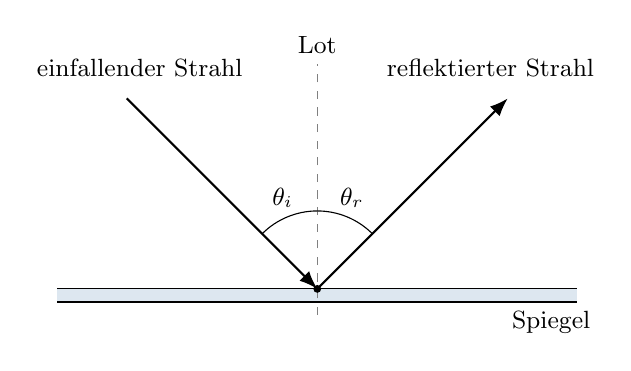
\begin{tikzpicture}[>=Latex, scale=1.1]
  \draw[thick] (-3,0) -- (3,0);
  \fill[kfrblue!15] (-3,-0.15) rectangle (3,0);
  \draw[thick] (-3,-0.15) -- (3,-0.15);
  \node[below] at (2.7,-0.15) {\small Spiegel};
  \draw[dashed, gray] (0,-0.3) -- (0,2.6);
  \node[above] at (0,2.6) {\small Lot};
  \draw[->, thick] (-2.2,2.2) -- (0,0);
  \node at (-2.05,2.55) {\small einfallender Strahl};
  \draw[->, thick] (0,0) -- (2.2,2.2);
  \node at (2.0,2.55) {\small reflektierter Strahl};
  \draw (0,0) ++(90:0.9) arc (90:135:0.9);
  \node at (-0.4,1.05) {\small $\theta_i$};
  \draw (0,0) ++(90:0.9) arc (90:45:0.9);
  \node at (0.4,1.05) {\small $\theta_r$};
  \node[circle,fill=black,inner sep=1pt] at (0,0) {};
\end{tikzpicture}
\end{center}

\subsection{Brechung}
Trifft Licht schräg auf die Grenzfläche zwischen zwei durchsichtigen Stoffen mit unterschiedlicher \textbf{Brechzahl} $n$ (auch Brechungsindex genannt, dimensionslos), so ändert es beim Übertritt seine Richtung: es wird \emph{gebrochen}. Auch hier misst man Einfallswinkel $\alpha$ und Brechungswinkel $\beta$ jeweils zum Lot. Es gilt das \textbf{Brechungsgesetz (Snellius)}:
\[
  n_1 \sin\alpha = n_2 \sin\beta.
\]
Für unseren Versuch ist Medium~1 Luft, mit $n_1 \approx 1$. Damit vereinfacht sich die Formel, und die gesuchte Brechzahl des Acrylglases ergibt sich direkt aus den beiden gemessenen Winkeln:
\[
  n_{\text{Acryl}} = \frac{\sin\alpha}{\sin\beta}.
\]

\begin{center}
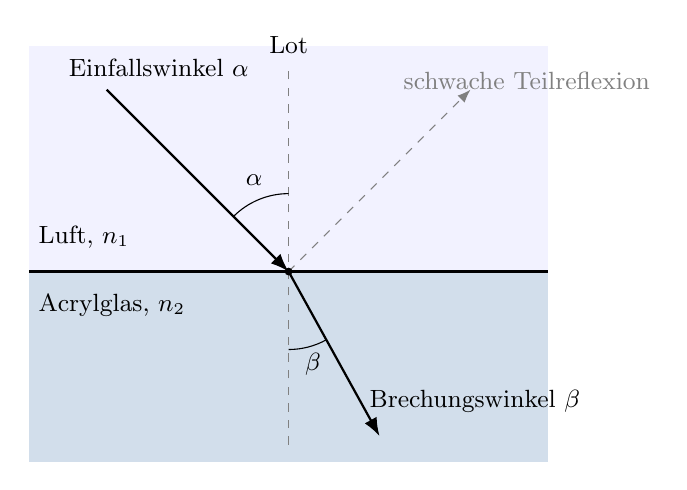
\begin{tikzpicture}[>=Latex, scale=1.1]
  \fill[blue!5] (-3,0) rectangle (3,2.6);
  \fill[kfrblue!20] (-3,-2.2) rectangle (3,0);
  \draw[thick] (-3,0) -- (3,0);
  \node[above right] at (-3,0.15) {\small Luft, $n_1$};
  \node[below right] at (-3,-0.15) {\small Acrylglas, $n_2$};
  \draw[dashed, gray] (0,-2.0) -- (0,2.4);
  \node[above] at (0,2.4) {\small Lot};
  \draw[->, thick] (-2.1,2.1) -- (0,0);
  \node at (-1.5,2.35) {\small Einfallswinkel $\alpha$};
  \draw[->, thick] (0,0) -- (1.05,-1.9);
  \node at (2.15,-1.5) {\small Brechungswinkel $\beta$};
  \draw[->, thin, gray, dashed] (0,0) -- (2.1,2.1);
  \node[gray] at (2.75,2.2) {\small schwache Teilreflexion};
  \draw (0,0) ++(90:0.9) arc (90:135:0.9);
  \node at (-0.4,1.05) {\small $\alpha$};
  \draw (0,0) ++(-90:0.9) arc (-90:-61:0.9);
  \node at (0.28,-1.07) {\small $\beta$};
  \node[circle,fill=black,inner sep=1pt] at (0,0) {};
\end{tikzpicture}
\end{center}

\begin{tippbox}
Weil $n_2 > n_1$ ist (Acrylglas ist optisch dichter als Luft), gilt beim Übertritt von Luft in Acrylglas immer $\beta < \alpha$: der Strahl wird zum Lot hin gebrochen. Am Übergang tritt zudem, wie in der Skizze angedeutet, immer ein schwacher Teil des Lichts auch reflektiert aus, nicht nur der Hauptanteil, der gebrochen wird.
\end{tippbox}

\subsection{Messunsicherheit: Fehlerarten}
\label{sec:fehlerarten}
Keine Messung ist perfekt exakt: Jeder Messwert hat eine gewisse \textbf{Messunsicherheit} $\Delta x$, auch Fehler genannt. Man unterscheidet drei Fehlerarten:
\begin{itemize}
  \item \textbf{Ablese- bzw.\ Auflösungsfehler:} entsteht, weil sich eine Skala nur bis zu einer gewissen Feinheit ablesen lässt (z.\,B.\ die Winkelskala des Drehtisches). Er lässt sich meist als halbe kleinste Skalenteilung abschätzen. Gibt es zwischen den Skalenstrichen aber keine feinere Unterteilung, an der sich ein halber Skalenteil plausibel ablesen lässt, wählt man stattdessen die volle kleinste Skalenteilung als Ablesegenauigkeit.
  \item \textbf{Zufälliger Fehler:} entsteht durch unkontrollierbare, von Messung zu Messung leicht unterschiedliche Einflüsse (z.\,B.\ minimal unterschiedliches Ablesen, kleine Erschütterungen). Er streut zufällig nach oben und unten um den wahren Wert; Mehrfachmessung und Mittelwertbildung verkleinern ihn.
  \item \textbf{Systematischer Fehler:} verschiebt alle Messwerte auf dieselbe Art in dieselbe Richtung (z.\,B.\ eine leicht verdrehte Winkelskala oder ein Lichtstrahl, der nicht exakt im Drehpunkt liegt). Mehrfachmessung mittelt ihn nicht weg; nur ein sorgfältiger Aufbau vermeidet ihn.
\end{itemize}

\subsection{Trendlinie (Ausgleichsgerade)}
\label{sec:trendlinie}
Trägt man mehrere Messpunkte in ein Diagramm ein und folgen sie erkennbar einem linearen Zusammenhang, lässt sich eine Gerade durch die Punktwolke legen, welche diesen Zusammenhang am besten beschreibt: die \textbf{Trendlinie}, auch \textbf{Ausgleichsgerade} genannt.

Beim Zeichnen von Hand gilt: Die Trendlinie muss nicht exakt durch den ersten oder letzten Punkt gehen, und schon gar nicht durch den Ursprung. Sie soll so gelegt werden, dass die Punkte insgesamt möglichst nahe an der Geraden liegen, mit ungefähr gleich vielen Punkten oberhalb wie unterhalb der Linie.

Aus der gezeichneten Trendlinie lassen sich zwei Grössen ablesen:
\begin{itemize}
  \item die \textbf{Steigung} $k$: Wählt zwei gut lesbare Punkte auf der gezeichneten Geraden (diese müssen keine Messpunkte sein) und berechnet $k = \dfrac{\Delta y}{\Delta x}$;
  \item der \textbf{Achsenabschnitt} $d$: der $y$-Wert, an dem die Trendlinie die $y$-Achse (bei $x=0$) schneidet.
\end{itemize}
Damit lässt sich die Trendlinie als Geradengleichung schreiben:
\[
  y = k\cdot x + d.
\]

\begin{center}
\begin{tikzpicture}[>=Latex, scale=0.85]
  \draw[->] (-0.6,0) -- (6.4,0) node[right] {\small $x$};
  \draw[->] (0,-0.6) -- (0,5.2) node[above] {\small $y$};
  \draw[kfrblue, thick] (0,1) -- (6,4.6) node[right] {\small $y=k\cdot x+d$};
  \draw[dashed, gray] (1,1.6) -- (4,1.6) -- (4,3.4);
  \node[below] at (2.5,1.6) {\small $\Delta x$};
  \node[right] at (4,2.5) {\small $\Delta y$};
  \fill[warnorange] (1,1.6) circle (2pt) node[above left] {\small $P_1$};
  \fill[warnorange] (4,3.4) circle (2pt) node[above left] {\small $P_2$};
  \draw[dashed, gray] (0,1) -- (0.15,1);
  \fill (0,1) circle (1.5pt) node[left] {\small $d$};
  \node[circle,fill=black,inner sep=0.8pt] at (0,0) {};
\end{tikzpicture}
\end{center}
Steigung und Achsenabschnitt ergeben sich aus zwei abgelesenen Punkten $P_1(x_1,y_1)$ und $P_2(x_2,y_2)$ auf der Geraden:
\[
  k = \frac{\Delta y}{\Delta x} = \frac{y_2-y_1}{x_2-x_1}, \qquad d = y_1 - k\cdot x_1.
\]

\begin{tippbox}
In eurer Messdatendatei ist in jedem der beiden Diagramme bereits automatisch eine Trendlinie eingezeichnet, sobald ihr Messwerte eingetragen habt: Excel berechnet sie exakt aus euren Punkten (lineare Regression). Ihr müsst diese Trendlinie nicht selbst erstellen, sie dient nur zum Vergleich mit eurer eigenen Handzeichnung auf Papier.
\end{tippbox}

\subsection{Fehlerrechnung: Fehler von Quotienten}
\label{sec:fehlerrechnung}
Viele physikalische Grössen werden als Quotient zweier gemessener Grössen berechnet, z.\,B.\ $k=\dfrac{a}{b}$. Für die Unsicherheit eines solchen Quotienten (oder Produkts) gilt folgende Regel (ohne Herleitung, nur zum Anwenden): Die \textbf{relativen} Fehler der beiden Messgrössen addieren sich.
\[
  \frac{\Delta k}{k} = \frac{\Delta a}{a} + \frac{\Delta b}{b}, \qquad \text{also} \qquad \Delta k = k\cdot\left(\frac{\Delta a}{a}+\frac{\Delta b}{b}\right).
\]
Das gilt für jeden einzelnen Messpunkt separat, ihr erhaltet also pro Punkt ein eigenes $k_i$ und $\Delta k_i$.

Habt ihr mehrere solche Einzelmessungen $k_i$ (z.\,B.\ einen pro Messpunkt), ist der Mittelwert $\bar k$ die beste Schätzung für das Endresultat. Der Fehler dieses Mittelwerts ergibt sich aus der quadratischen Kombination aller Einzelfehler (ohne Herleitung):
\[
  \bar k = \frac{1}{N}\sum_i k_i, \qquad \Delta \bar k = \frac{1}{N}\sqrt{\sum_i (\Delta k_i)^2}.
\]

\begin{aufgabebox}
Recherchiert im Internet, wo Reflexion und Brechung in Technik oder Alltag eine wichtige Rolle spielen. Nennt mindestens zwei Beispiele und erklärt sie kurz.
\end{aufgabebox}
\zeichenraum[4.8cm]
\begin{solution}
\begin{loesungbox}
Zum Beispiel: (1) \textbf{Brillen und Kameraobjektive} nutzen gezielt geschliffene Linsen, um Licht durch Brechung zu bündeln bzw.\ zu streuen und so ein scharfes Bild zu erzeugen. (2) \textbf{Glasfaserkabel} (Lichtwellenleiter) leiten Licht über sehr viele Totalreflexionen an der Grenzfläche fast verlustfrei über lange Strecken, das Grundprinzip moderner Internet- und Telefonleitungen. Weitere mögliche Beispiele: Rückspiegel/Verkehrsspiegel (Reflexion), Regenbogen (Brechung und Reflexion in Wassertropfen), reflektierende Leitplanken oder Kleidung (Reflexion für Sicherheit im Strassenverkehr).
\end{loesungbox}
\end{solution}

% ======================================================
\section{Sicherheitshinweise}
\begin{itemize}
  \item Die Lichtquelle wird über ein Verlängerungskabel mit Strom versorgt: Kabel so verlegen, dass niemand darüber stolpert.
  \item Nicht direkt in den Lichtstrahl bzw.\ in die Lichtquelle blicken.
  \item Die Lampe der Lichtquelle kann nach längerem Betrieb warm werden: nicht direkt am Lampengehäuse anfassen.
\end{itemize}

% ======================================================
\section{Material}
Pro Gruppe ein vollständiger PASCO-Optikbaukasten:
\begin{itemize}
  \item Lichtquelle mit Spaltblende
  \item Drehtisch mit Winkelskala
  \item Spiegel
  \item Halbzylinder aus Acrylglas
  \item Verlängerungskabel
\end{itemize}
Jede Gruppe arbeitet mit ihrem eigenen, vollständigen Baukasten.

\begin{center}
  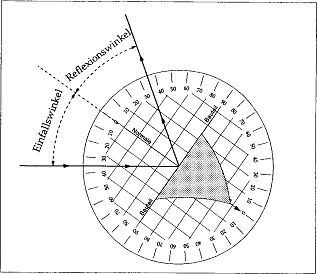
\includegraphics[width=0.5\linewidth]{Bilder/nahaufnahme_drehtisch.jpeg}\\
  {\small\itshape Nahaufnahme des Drehtisches mit Winkelskala.}
\end{center}

% ======================================================
\section{Planung}
\begin{aufgabebox}[{ (Plenum)}]
Diskutiert gemeinsam, bevor ihr mit dem Aufbau beginnt:
\begin{itemize}
  \item Wie erreicht ihr einen möglichst dünnen, scharf begrenzten Lichtstrahl auf dem Drehtisch? (Tipp: Position des Drehtisches auf der Schiene.)
  \item Wie verhindert ihr störendes Streulicht neben dem eigentlichen Lichtstrahl?
  \item Was passiert, wenn Spiegel oder Halbzylinder nicht exakt im Drehpunkt stehen?
  \item Warum messt ihr jeden Winkel zweimal: einmal mit dem einfallenden Strahl links und einmal rechts vom Lot?
\end{itemize}
\end{aufgabebox}
\zeichenraum[5.6cm]
\begin{solution}
\begin{loesungbox}
\begin{itemize}
  \item Ein dünner, scharfer Strahl entsteht, wenn der Drehtisch möglichst nah an der Spaltblende steht (der Lichtstrahl divergiert sonst sichtbar) und die Spaltblende sauber fokussiert eingestellt ist.
  \item Streulicht wird durch Abdunkeln des Raums und durch eine sauber ausgerichtete Spaltblende reduziert.
  \item Stehen Spiegel oder Halbzylinder nicht exakt im Drehpunkt, verschiebt sich der Auftreffpunkt beim Drehen des Tisches: Der abgelesene Winkel stimmt dann nicht mehr mit dem tatsächlichen Einfalls-, Reflexions- bzw.\ Brechungswinkel überein (systematischer Fehler).
  \item Ein Justierfehler der Spiegelebene (z.\,B.\ eine leicht verdrehte Skala oder ein schief stehender Spiegel) verschiebt den links gemessenen Winkel um einen bestimmten Betrag nach oben und den rechts gemessenen Winkel um denselben Betrag nach unten (oder umgekehrt). Beim Mitteln beider Werte hebt sich dieser systematische Fehler exakt weg, weshalb die Messung links und rechts vom Lot genauer ist als eine einzelne Messung.
\end{itemize}
\end{loesungbox}
\end{solution}

% ======================================================
\section{Durchführung}
Eure Messwerte tragt ihr direkt in die Datei \texttt{09EmmN\_Messdaten\_Reflexion\_Brechung.xlsx} ein. Sie enthält drei Blätter: Lest zuerst das Blatt „Hinweise“, dort ist die Farblegende erklärt: \textbf{gelb} hinterlegte Zellen tragt ihr selbst ein (Messwerte und eure Handrechnung), \textbf{blau} hinterlegte Zellen berechnen sich automatisch aus euren Eingaben (nicht überschreiben), \textbf{grün} hinterlegte Zellen zeigen automatisch berechnete Vergleichswerte zum Abgleich mit eurer Handrechnung. Auf dem Anleitungsblatt selbst werden keine Messwerttabellen mehr geführt.

\subsection{Reflexion}
\begin{center}
  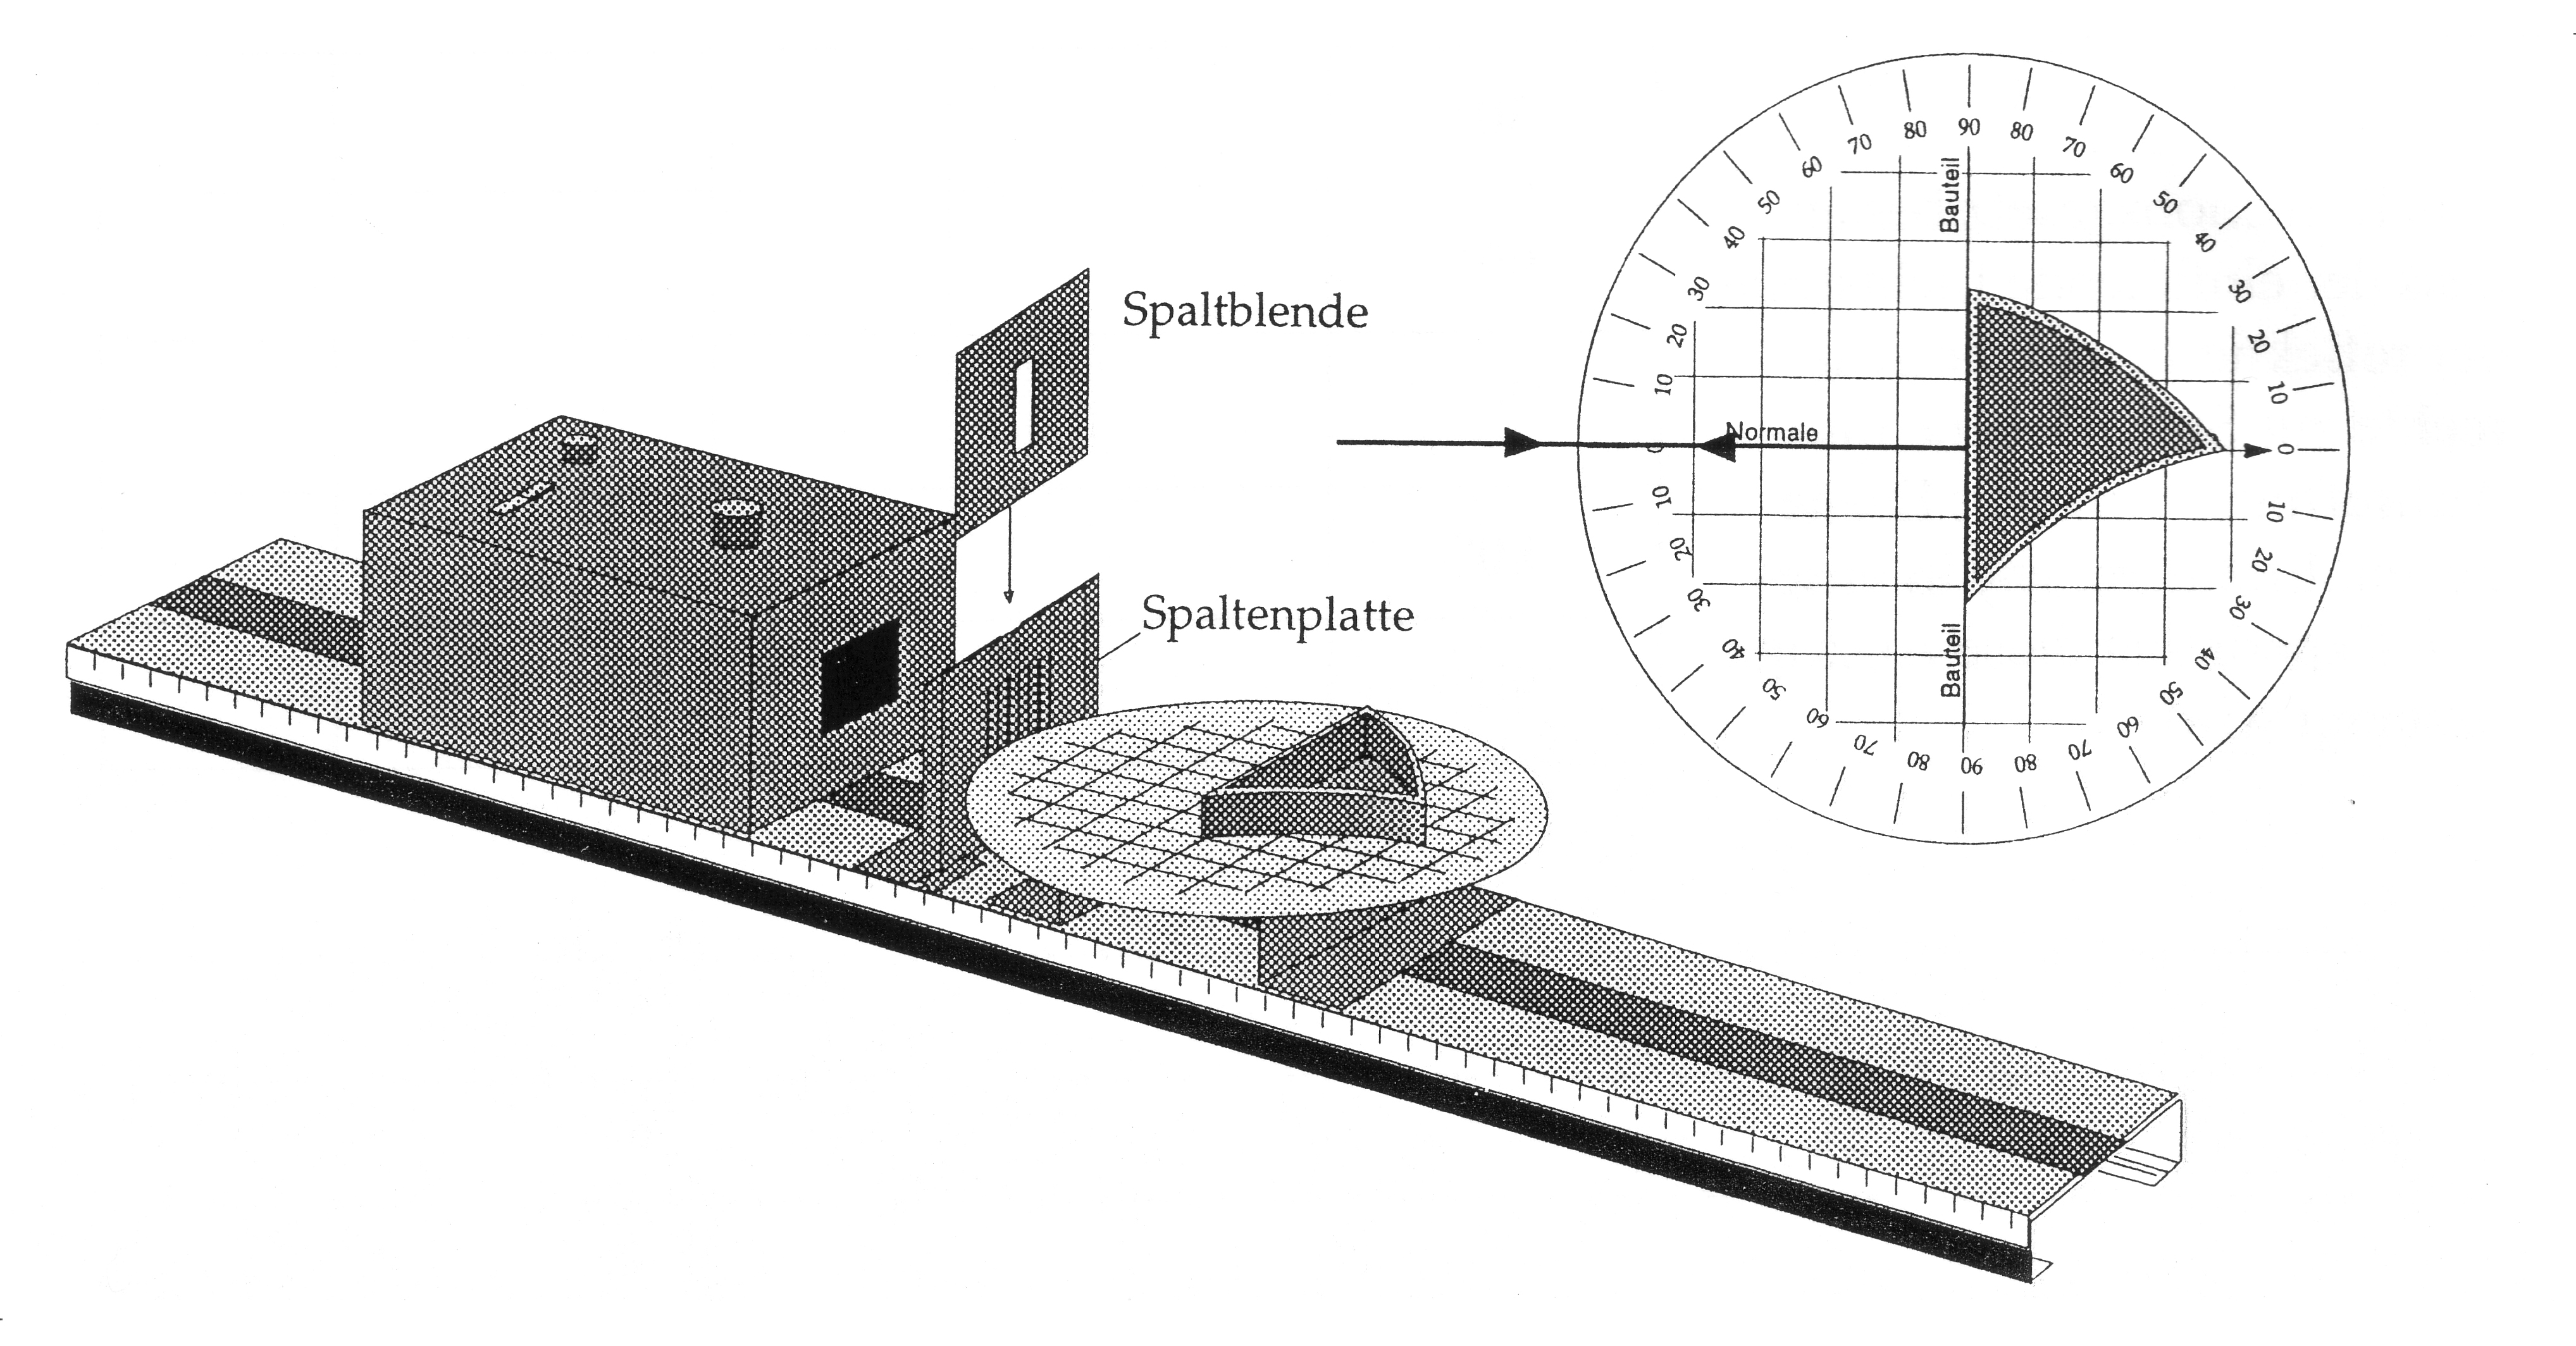
\includegraphics[width=0.6\linewidth]{Bilder/aufbau_reflexion.jpeg}\\
  {\small\itshape Aufbau für die Reflexionsmessung: Lichtquelle, Drehtisch mit Winkelskala, Spiegel.}
\end{center}

\begin{enumerate}
  \item Baut Lichtquelle, Drehtisch und Spiegel gemäss eurer Planung auf (siehe Abschnitt~4).
  \item Kontrolliert die Ausrichtung: Stellt einen Einfallswinkel von $0^\circ$ ein. Einfallender und reflektierter Strahl müssen dabei exakt zusammenfallen (auf derselben Linie zurücklaufen). Ist das nicht der Fall, justiert Spiegel oder Drehtisch nach, bevor ihr weitermesst.
  \item Öffnet im Excel das Blatt „Reflexion“. In Spalte A (Zeilen 5--14) sind die zehn zu untersuchenden Einfallswinkel bereits vorgegeben: $0^\circ, 10^\circ, 20^\circ, \dots, 90^\circ$. Stellt am Drehtisch nacheinander jeden dieser Winkel ein.
  \item Lest bei jedem Einfallswinkel den Reflexionswinkel zweimal ab: einmal mit dem einfallenden Strahl links vom Lot (Spalte B), einmal rechts vom Lot (Spalte D).
  \item Spalte F (Mittelwert des Reflexionswinkels) füllt sich automatisch, sobald B und D ausgefüllt sind.
\end{enumerate}

\subsection{Brechung}
\begin{center}
  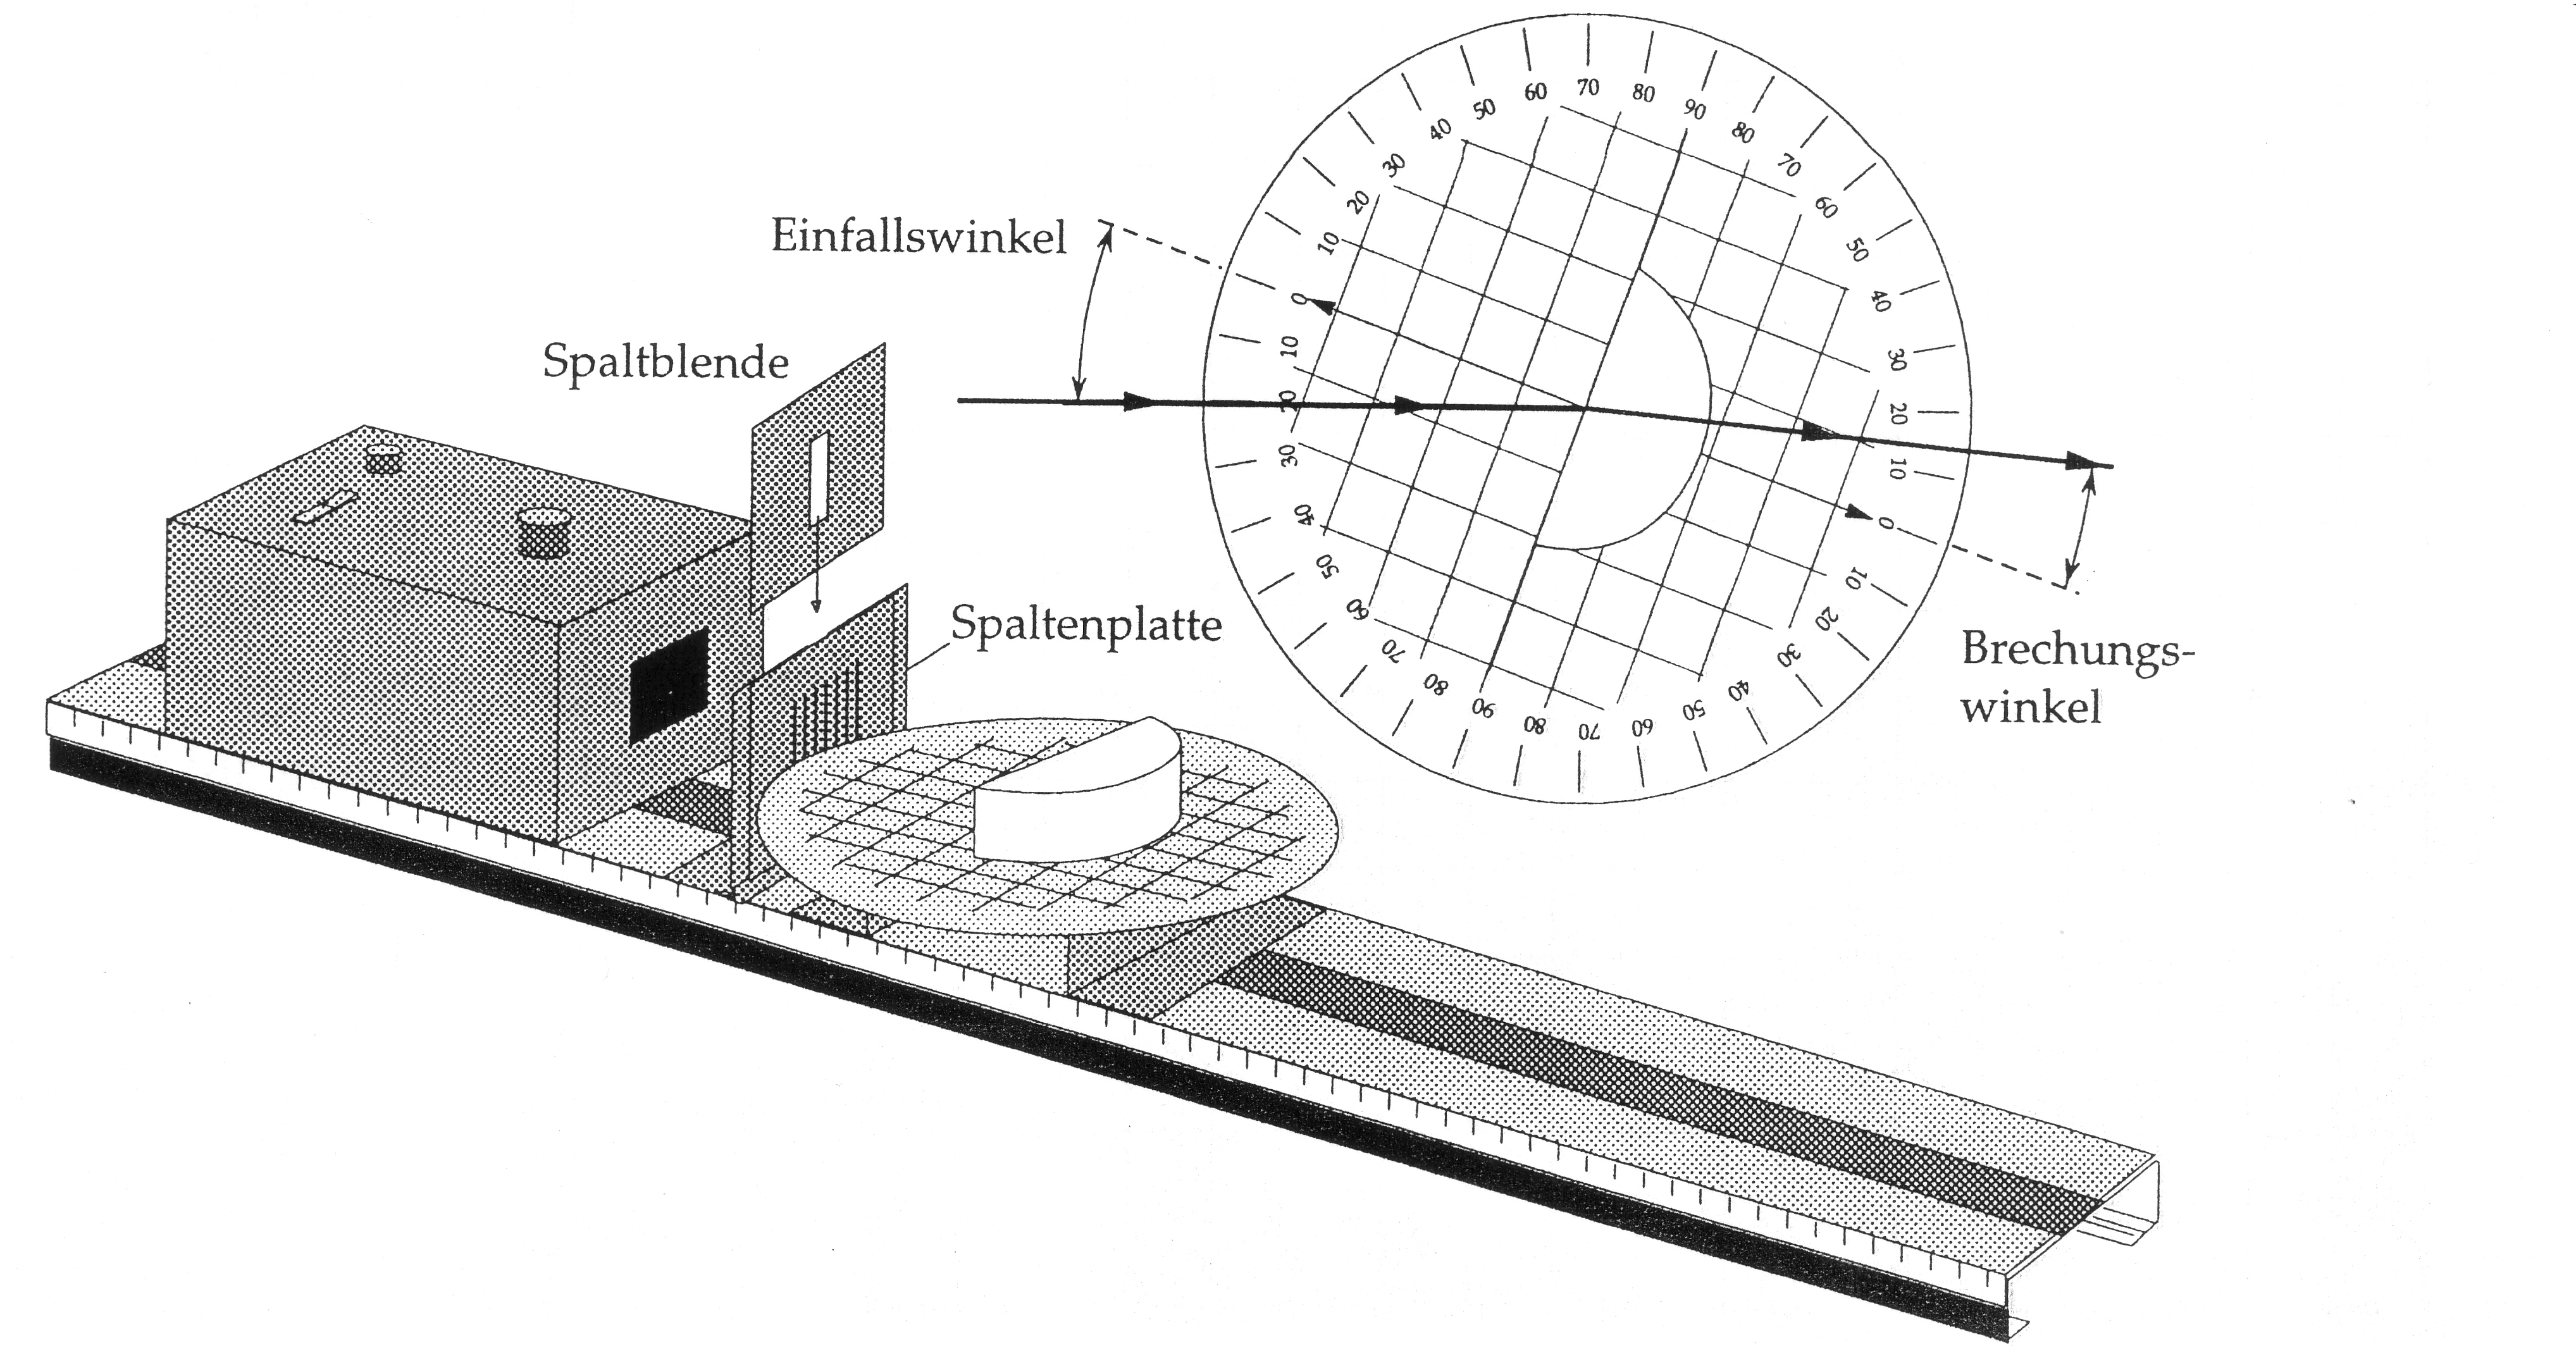
\includegraphics[width=0.6\linewidth]{Bilder/aufbau_brechung.jpeg}\\
  {\small\itshape Aufbau für die Brechungsmessung: Lichtquelle, Drehtisch mit Winkelskala, Acrylglaskörper.}
\end{center}

\begin{enumerate}
  \item Ersetzt den Spiegel durch den Halbzylinder aus Acrylglas, so dass der Lichtstrahl zuerst auf die flache Seite trifft, und zwar genau im Drehpunkt (Mittelpunkt der Kreisfläche); er tritt anschliessend an der gekrümmten Seite wieder aus.
  \item Öffnet das Blatt „Brechung“. Auch hier sind in Spalte A (Zeilen 5--14) die zehn Einfallswinkel $\alpha$ vorgegeben ($0^\circ$ bis $90^\circ$ in $10^\circ$-Schritten).
  \item Berechnet für jeden Winkel $\sin\alpha$ von Hand mit dem Taschenrechner und tragt den Wert in Spalte B ein.
  \item Stellt am Drehtisch den jeweiligen Einfallswinkel ein und lest den Brechungswinkel zweimal ab: links vom Lot in Spalte C, rechts vom Lot in Spalte E.
  \item Spalte G (Mittelwert von $\beta$) füllt sich automatisch. Berechnet daraus $\sin\beta$ von Hand und tragt den Wert in Spalte I ein. Spalte J zeigt euch dann automatisch die Brechzahl $n$ für diesen einzelnen Messpunkt.
\end{enumerate}

\begin{achtungbox}
Stellt euren Taschenrechner auf \textbf{DEG} (Grad) um, bevor ihr $\sin\alpha$ und $\sin\beta$ berechnet. Im falschen Winkelmodus (RAD oder GRAD) erhaltet ihr sinnlose Werte, ohne dass der Taschenrechner eine Fehlermeldung zeigt.
\end{achtungbox}

\begin{aufgabebox}
Bei grossen Einfallswinkeln bemerkt ihr eventuell einen schwachen, reflektiert wirkenden Strahl, obwohl ihr eigentlich die Brechung untersucht. Woher kommt dieser Strahl? Ist er nur bei grossen Winkeln vorhanden, oder auch bei kleinen (nur weniger sichtbar)? \textbf{Tipp: Raum dunkel machen!} Der schwache Strahl ist sonst kaum zu erkennen.
\end{aufgabebox}
\zeichenraum[4cm]
\begin{solution}
\begin{loesungbox}
Der schwache Strahl ist eine \textbf{Teilreflexion} an der Grenzfläche: Ein kleiner Teil des Lichts wird immer reflektiert, auch wenn der Hauptanteil gebrochen wird (vgl.\ Merkbox in Abschnitt~2.2). Dieser Effekt ist bei jedem Winkel vorhanden, bei kleinen Einfallswinkeln aber so schwach, dass er kaum auffällt; bei grossen Einfallswinkeln (nahe der streifenden Inzidenz) wird der reflektierte Anteil deutlich stärker und damit gut sichtbar. Der Grund: Je flacher das Licht auf die Grenzfläche trifft, desto grösser ist der Anteil, der reflektiert statt gebrochen wird. Bei streifendem Einfall (Einfallswinkel nahe $90^\circ$) wird sogar praktisch das gesamte Licht reflektiert, unabhängig vom Material, das Acrylglas verhält sich dann fast wie ein Spiegel.
\end{loesungbox}
\end{solution}

\begin{aufgabebox}
Verschiebt den Halbzylinder absichtlich leicht so, dass der Lichtstrahl nicht mehr exakt durch den Mittelpunkt der Kreisfläche (den Drehpunkt) trifft. Beobachtet, was mit dem gebrochenen Strahl passiert, und notiert eure Beobachtung.
\end{aufgabebox}
\zeichenraum[4cm]
\begin{solution}
\begin{loesungbox}
An der flachen Fläche selbst ändert sich zunächst wenig: Sie hat überall dieselbe Flächennormale, die Brechung dort folgt weiterhin korrekt dem eingestellten Einfallswinkel $\alpha$. Das Problem entsteht beim Austritt: Der gebrochene Strahl verläuft im Glas nur dann entlang eines Radius zur gekrümmten Fläche (und trifft dort senkrecht, ohne weitere Richtungsänderung), wenn er exakt durch den Mittelpunkt der Kreisfläche eingetreten ist. Trifft der Strahl daneben, erreicht er die gekrümmte Fläche nicht mehr senkrecht und wird dort ein zweites Mal gebrochen. Der am äusseren Drehtisch abgelesene Winkel entspricht dann nicht mehr dem tatsächlichen Brechungswinkel $\beta$ an der flachen Grenzfläche: Die einfache Formel $n=\sin\alpha/\sin\beta$ liefert einen falschen Wert. Deshalb muss der Strahl exakt durch den Drehpunkt laufen, nur dann bleibt die gekrümmte Fläche beim Austritt wirkungslos und die gesamte Brechung findet, wie in der Theorie angenommen, ausschliesslich an der flachen Grenzfläche statt.
\end{loesungbox}
\end{solution}

% ======================================================
\section{Auswertung}
\label{sec:auswertung}
Die Fehlerrechnung erfolgt in vier Schritten. Schritt~1 (Messunsicherheit) macht ihr einmal für den ganzen Versuch; die Schritte~2--4 macht ihr separat für Reflexion und Brechung.

\subsection{Schritt 1: Messunsicherheit $\Delta\theta$ bestimmen}
\begin{aufgabebox}
Bestimmt eure Ablesegenauigkeit an der Winkelskala $\Delta\theta_{\text{Skala}}$ (wie fein könnt ihr den Winkel wirklich noch unterscheiden, vgl.\ Abschnitt~\ref{sec:fehlerarten}?) und schätzt zusätzlich die Winkelbreite des Lichtstrahls selbst $\Delta\theta_{\text{Strahl}}$ ab: Der Strahl ist kein unendlich dünner Strich, wie breit erscheint er auf der Skala, in Grad?
\end{aufgabebox}
\zeichenraum[3.2cm]
\begin{solution}
\begin{loesungbox}
Beispielwerte: $\Delta\theta_{\text{Skala}} \approx 1^\circ$ (vgl.\ Abschnitt~4). Der Lichtstrahl erscheint auf der Skala je nach Spaltbreite und Fokussierung typischerweise ebenfalls rund $1^\circ$ breit, also $\Delta\theta_{\text{Strahl}} \approx 1^\circ$.
\end{loesungbox}
\end{solution}

Die beiden Fehlerquellen kombiniert ihr zu einer gemeinsamen Messunsicherheit pro Winkelablesung (Summenregel):
\[
  \Delta\theta = \Delta\theta_{\text{Skala}} + \Delta\theta_{\text{Strahl}}.
\]
Tragt $\Delta\theta_{\text{Skala}}$, $\Delta\theta_{\text{Strahl}}$ und $\Delta\theta$ im Blatt „Reflexion“ in die gelben Zellen C45--C47 \emph{und} im Blatt „Brechung“ in die gelben Zellen C46--C48 ein (denselben Wert, Excel benötigt ihn separat auf jedem Blatt).

\subsection{Schritt 2: Graph von Hand zeichnen, Steigung ablesen}

\textbf{Reflexion.} Erwartete Geradengleichung: $\theta_r = k\cdot\theta_i + d$. Übertrage deine zehn Messpunkte von Hand in das Diagramm ein: Einfallswinkel (Spalte A) auf die $x$-Achse, gemittelter Reflexionswinkel (Spalte F) auf die $y$-Achse. Achsen und Skala sind bereits eingezeichnet.
\begin{center}
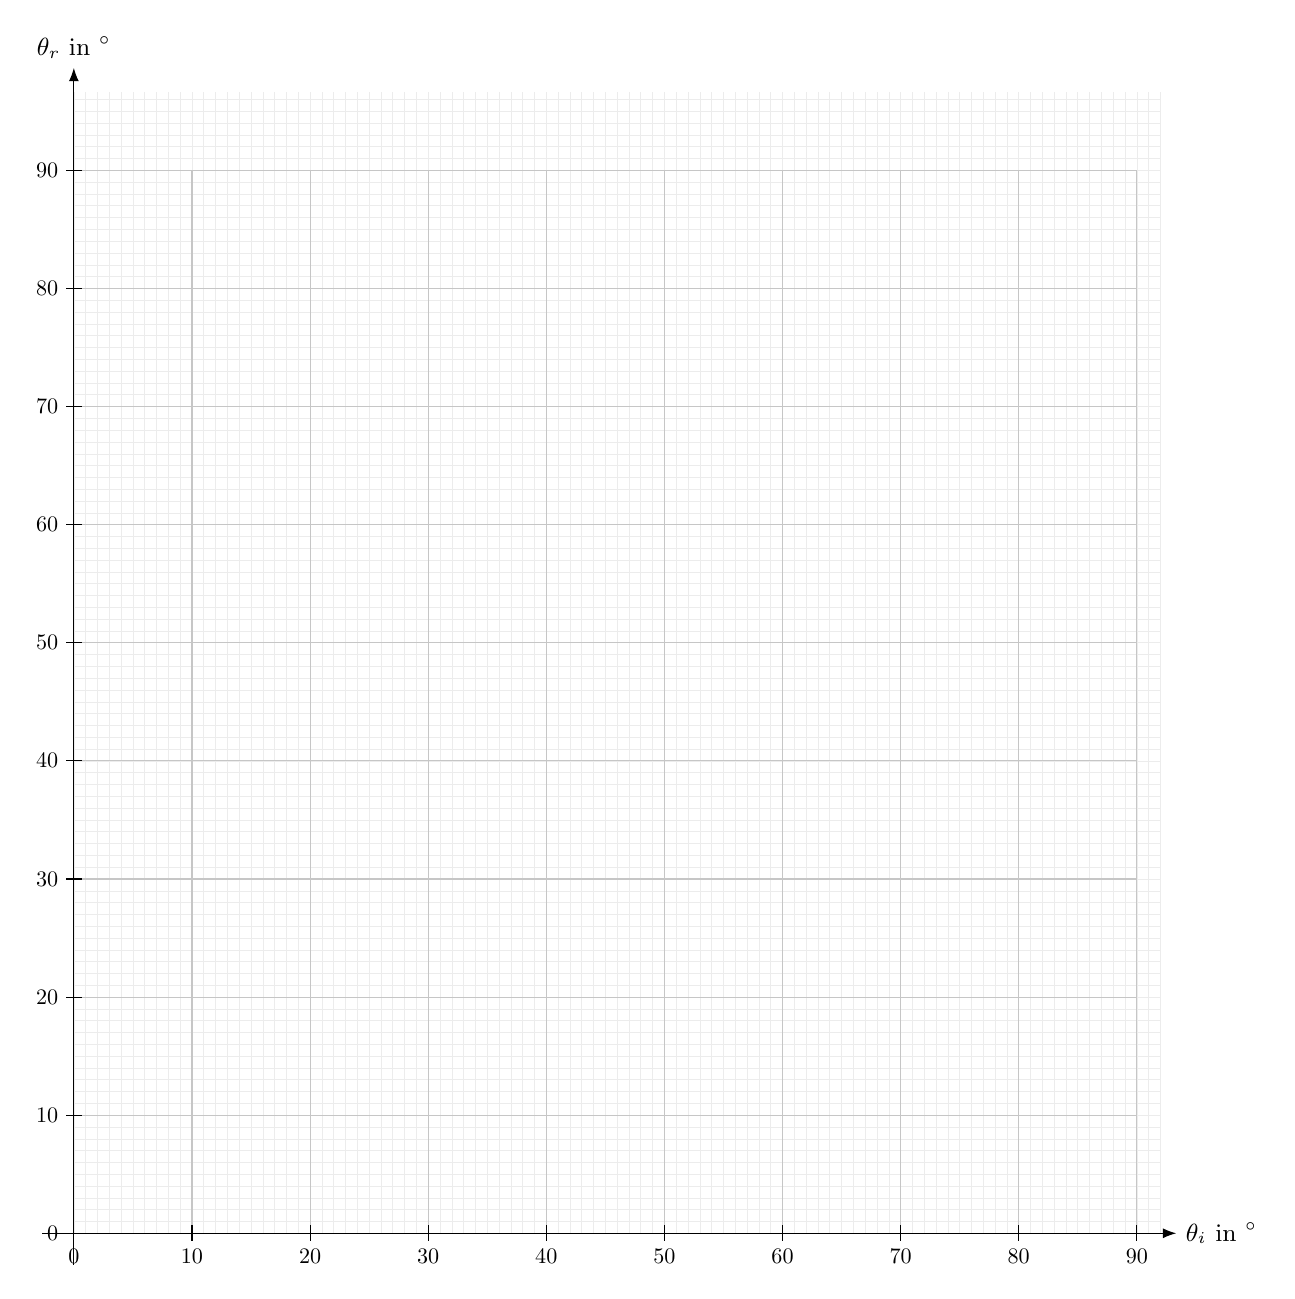
\begin{tikzpicture}[>=Latex]
  \draw[step=0.15cm, gray!15, very thin] (0,0) grid (13.8,14.5);
  \draw[step=1.5cm, gray!45, thin] (0,0) grid (13.5,13.5);
  \draw[->] (-0.4,0) -- (14.0,0) node[right] {\small $\theta_i$ in $^\circ$};
  \draw[->] (0,-0.4) -- (0,14.8) node[above] {\small $\theta_r$ in $^\circ$};
  \foreach \i/\lbl in {0/0,1.5/10,3.0/20,4.5/30,6.0/40,7.5/50,9.0/60,10.5/70,12.0/80,13.5/90} {
    \draw (\i,0.1) -- (\i,-0.1);
    \node[below, scale=0.8] at (\i,-0.1) {\lbl};
    \draw (0.1,\i) -- (-0.1,\i);
    \node[left, scale=0.8] at (-0.1,\i) {\lbl};
  }
\end{tikzpicture}
\end{center}
\begin{solution}
\noindent\textbf{\color{tipgreen}Lösung (Beispieldiagramm aus Testdaten):}
\begin{center}
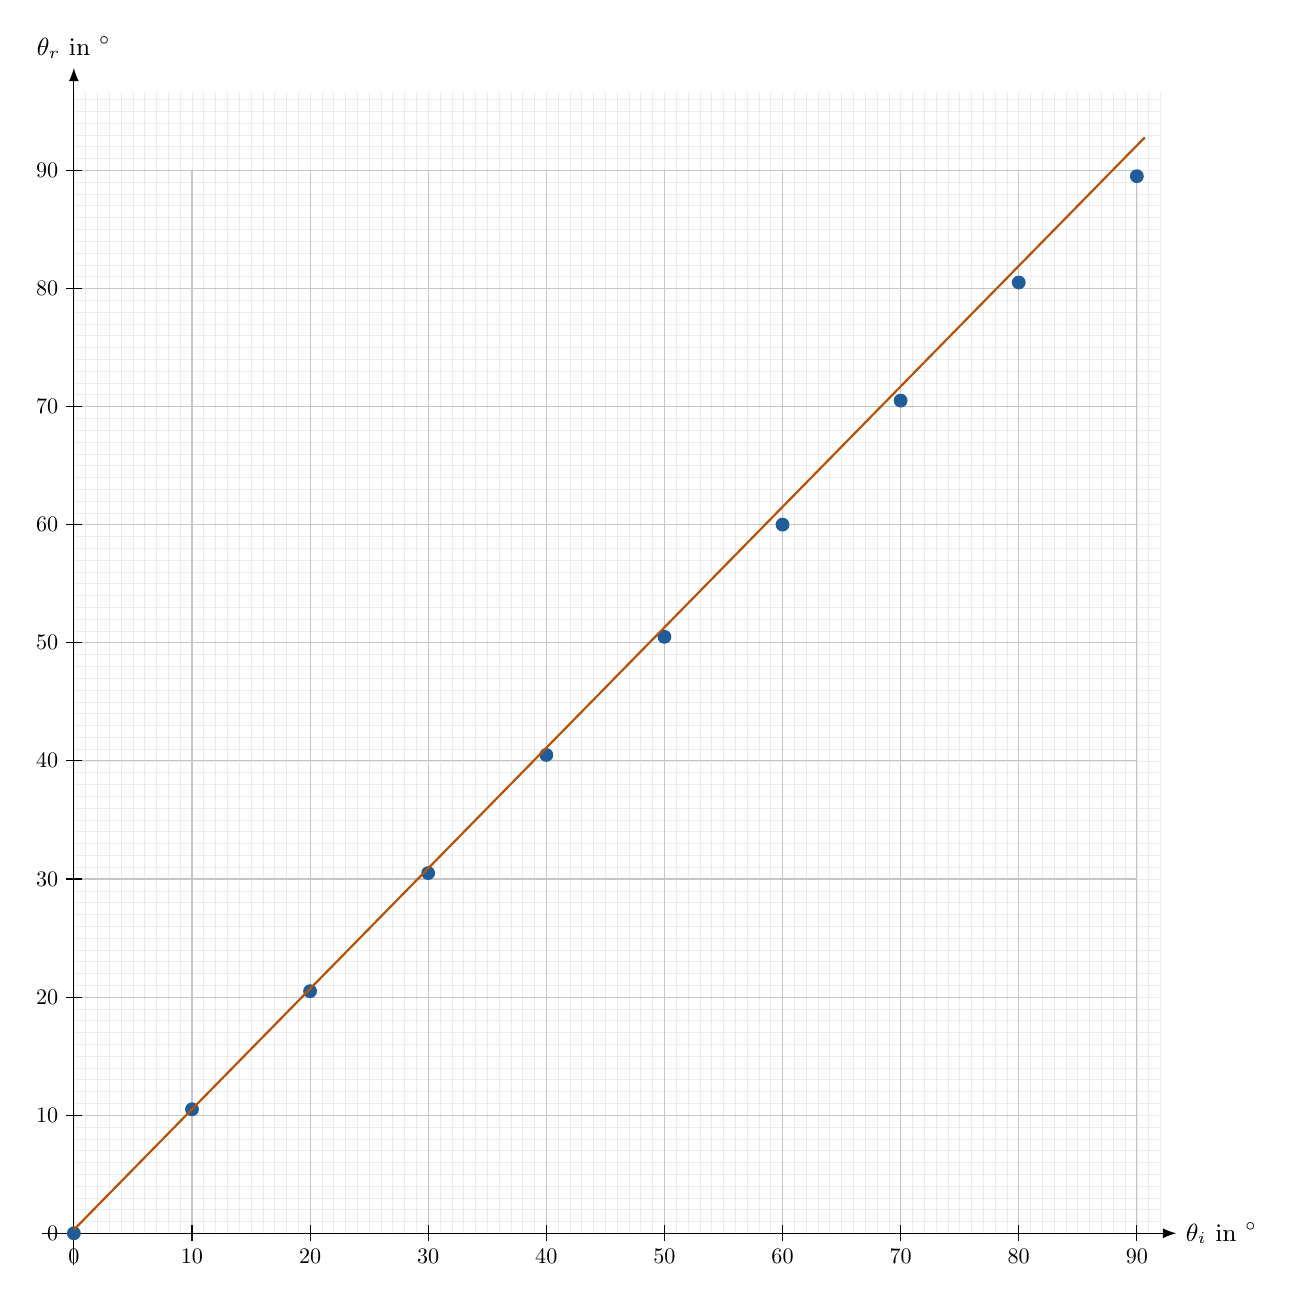
\begin{tikzpicture}[>=Latex]
  \draw[step=0.15cm, gray!15, very thin] (0,0) grid (13.8,14.5);
  \draw[step=1.5cm, gray!45, thin] (0,0) grid (13.5,13.5);
  \draw[->] (-0.4,0) -- (14.0,0) node[right] {\small $\theta_i$ in $^\circ$};
  \draw[->] (0,-0.4) -- (0,14.8) node[above] {\small $\theta_r$ in $^\circ$};
  \foreach \i/\lbl in {0/0,1.5/10,3.0/20,4.5/30,6.0/40,7.5/50,9.0/60,10.5/70,12.0/80,13.5/90} {
    \draw (\i,0.1) -- (\i,-0.1);
    \node[below, scale=0.8] at (\i,-0.1) {\lbl};
    \draw (0.1,\i) -- (-0.1,\i);
    \node[left, scale=0.8] at (-0.1,\i) {\lbl};
  }
  \foreach \x/\y in {0/0, 1.5/1.575, 3.0/3.075, 4.5/4.575, 6.0/6.075, 7.5/7.575, 9.0/9.0, 10.5/10.575, 12.0/12.075, 13.5/13.425}
    \fill[kfrblue] (\x,\y) circle (2.5pt);
  \draw[warnorange, thick] (0,0.045) -- (13.6,13.917);
\end{tikzpicture}
\end{center}
\end{solution}

Zeichne die beste Gerade von Hand durch deine Punkte. Wähle zwei gut lesbare Punkte auf dieser Geraden (müssen keine Messpunkte sein) und berechne mit dem Steigungsdreieck (Abschnitt~\ref{sec:trendlinie}):
\[
  k = \frac{y_2-y_1}{x_2-x_1}, \qquad d = y_1 - k\cdot x_1.
\]
Tragt $k$ und $d$ im Blatt „Reflexion“ in die gelben Zellen C37--C38 ein.
\begin{solution}
\begin{loesungbox}
Abgelesen aus der Handzeichnung (Beispiel): $k \approx 1.02$, $d \approx 0.3^\circ$.
\end{loesungbox}
\end{solution}

\textbf{Brechung.} Snellius'sches Brechungsgesetz umgestellt: $\sin\alpha = n\cdot\sin\beta$, also Geradengleichung $\sin\alpha = k\cdot\sin\beta + d$ mit $k=n$. Damit die Steigung direkt die gesuchte Brechzahl $n$ ergibt (statt $1/n$), trägt ihr $\sin\beta$ (Spalte I) auf die $x$-Achse und $\sin\alpha$ (Spalte B) auf die $y$-Achse auf. Achsen und Skala sind bereits eingezeichnet.
\begin{center}
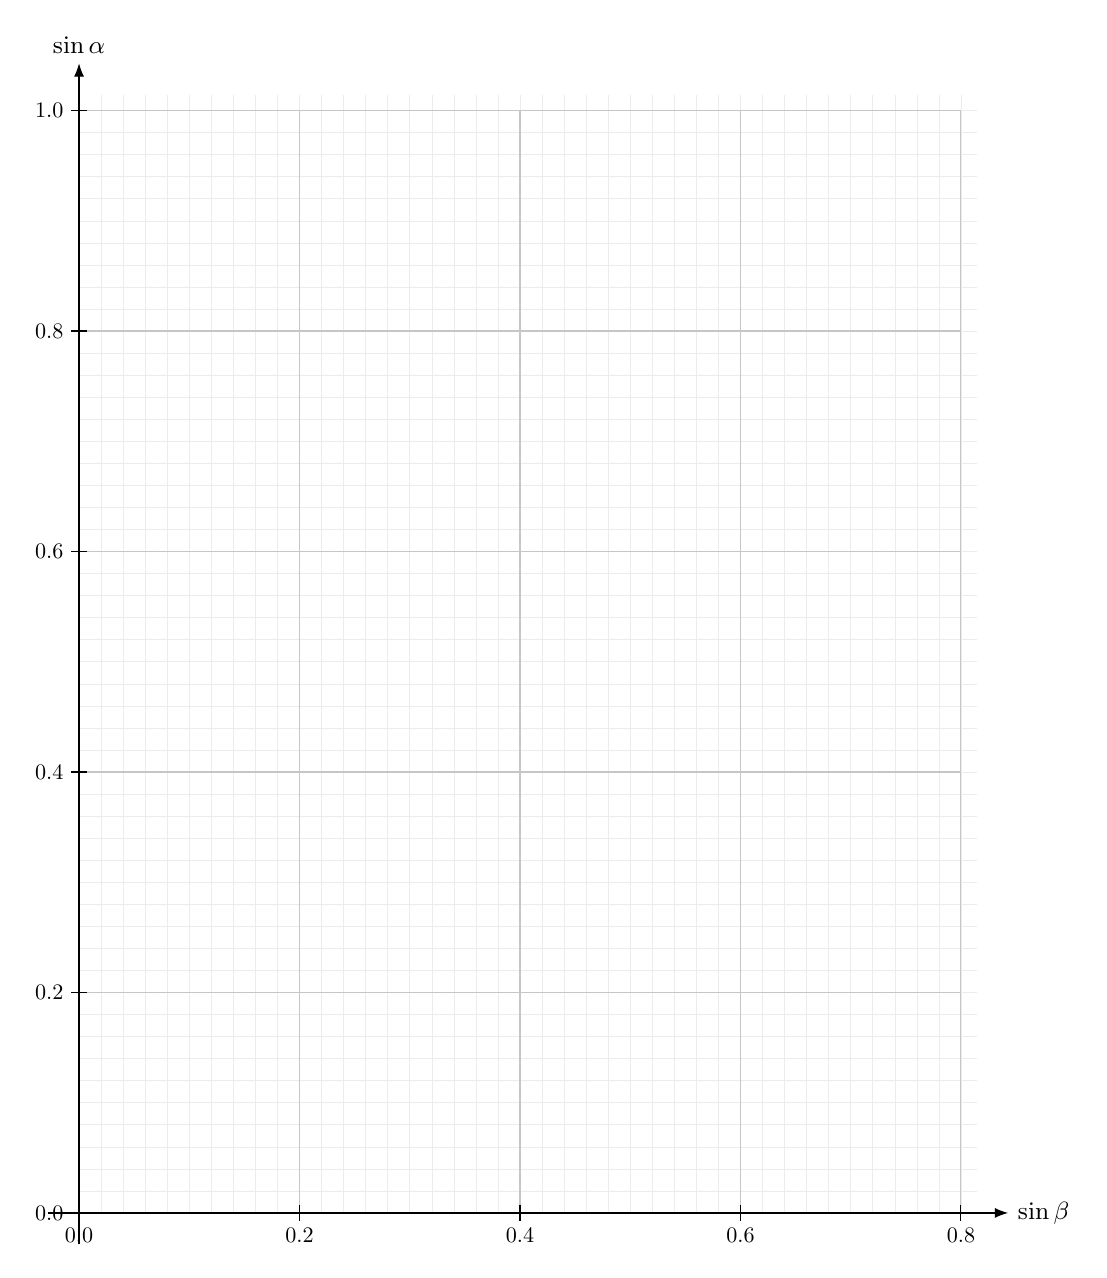
\begin{tikzpicture}[>=Latex]
  \draw[step=0.28cm, gray!15, very thin] (0,0) grid (11.4,14.2);
  \draw[step=2.8cm, gray!45, thin] (0,0) grid (11.2,14.0);
  \draw[->] (-0.4,0) -- (11.8,0) node[right] {\small $\sin\beta$};
  \draw[->] (0,-0.4) -- (0,14.6) node[above] {\small $\sin\alpha$};
  \foreach \i/\lbl in {0/0.0,2.8/0.2,5.6/0.4,8.4/0.6,11.2/0.8} {
    \draw (\i,0.1) -- (\i,-0.1);
    \node[below, scale=0.8] at (\i,-0.1) {\lbl};
  }
  \foreach \i/\lbl in {0/0.0,2.8/0.2,5.6/0.4,8.4/0.6,11.2/0.8,14.0/1.0} {
    \draw (0.1,\i) -- (-0.1,\i);
    \node[left, scale=0.8] at (-0.1,\i) {\lbl};
  }
\end{tikzpicture}
\end{center}
\begin{solution}
\noindent\textbf{\color{tipgreen}Lösung (Beispieldiagramm aus Testdaten):}
\begin{center}
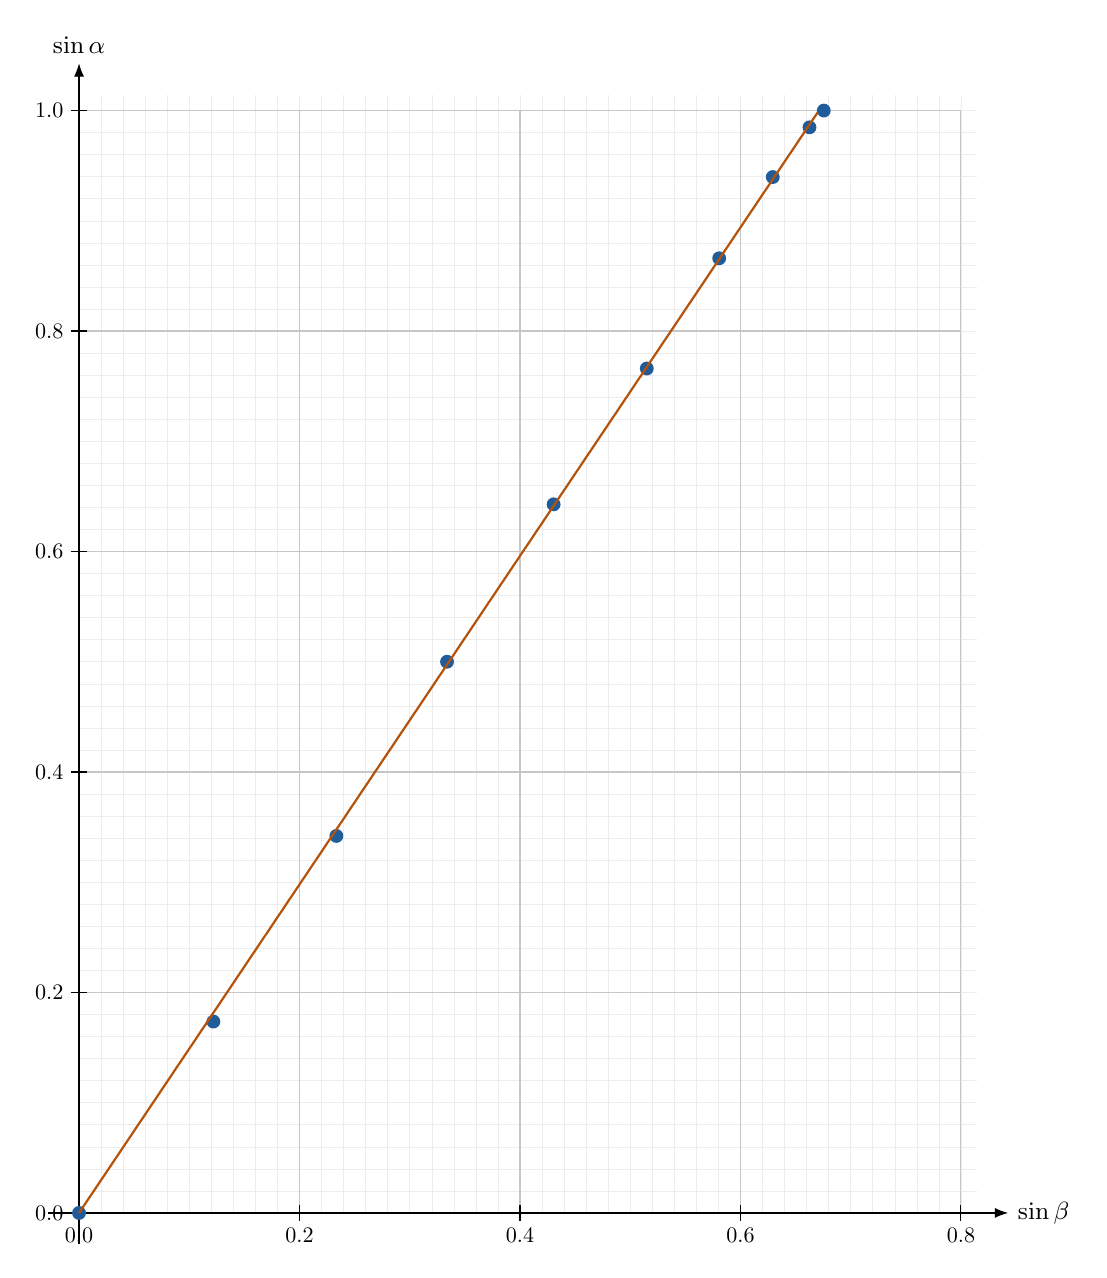
\begin{tikzpicture}[>=Latex]
  \draw[step=0.28cm, gray!15, very thin] (0,0) grid (11.4,14.2);
  \draw[step=2.8cm, gray!45, thin] (0,0) grid (11.2,14.0);
  \draw[->] (-0.4,0) -- (11.8,0) node[right] {\small $\sin\beta$};
  \draw[->] (0,-0.4) -- (0,14.6) node[above] {\small $\sin\alpha$};
  \foreach \i/\lbl in {0/0.0,2.8/0.2,5.6/0.4,8.4/0.6,11.2/0.8} {
    \draw (\i,0.1) -- (\i,-0.1);
    \node[below, scale=0.8] at (\i,-0.1) {\lbl};
  }
  \foreach \i/\lbl in {0/0.0,2.8/0.2,5.6/0.4,8.4/0.6,11.2/0.8,14.0/1.0} {
    \draw (0.1,\i) -- (-0.1,\i);
    \node[left, scale=0.8] at (-0.1,\i) {\lbl};
  }
  \foreach \x/\y in {0/0, 1.7062/2.4304, 3.2682/4.788, 4.6733/7.0, 6.0272/8.9992, 7.2105/10.724, 8.1298/12.124, 8.8105/13.1558, 9.2767/13.7872, 9.4583/14.0}
    \fill[kfrblue] (\x,\y) circle (2.5pt);
  \draw[warnorange, thick] (0,0) -- (9.38,13.976);
\end{tikzpicture}
\end{center}
\end{solution}

Zeichne die beste Gerade von Hand durch deine Punkte und berechne mit dem Steigungsdreieck $k$ und $d$ wie oben. Tragt eure Werte im Blatt „Brechung“ in die gelben Zellen C37--C38 ein: $k$ ist bereits eure gemessene Brechzahl $n$, keine weitere Umrechnung nötig.
\begin{solution}
\begin{loesungbox}
Abgelesen aus der Handzeichnung (Beispiel): $k=n \approx 1.49$, $d \approx 0.00$.
\end{loesungbox}
\end{solution}

\subsection{Schritt 3: Fehlerrechnung pro Messpunkt, dann Mittelung}

Grundidee: Statt nur die ganze Gerade zu betrachten, wendet ihr die Quotientenregel aus Abschnitt~\ref{sec:fehlerrechnung} für \textbf{jeden einzelnen} Messpunkt an und mittelt danach. So nutzt ihr wirklich alle zehn Messungen, mit Werkzeugen, die ihr schon kennt.

\textbf{Reflexion.} Formel pro Messpunkt (Quotientenregel):
\[
  k_i = \frac{\theta_{r,i}}{\theta_{i,i}}, \qquad \Delta k_i = k_i\left(\frac{\Delta\theta}{\theta_{r,i}}+\frac{\Delta\theta}{\theta_{i,i}}\right).
\]

\begin{aufgabebox}
Berechnet $k_i$ und $\Delta k_i$ für jeden Messpunkt \textbf{ausser} $\theta_i=0^\circ$ (dort könnt ihr nicht durch $0$ teilen; nennt selbst einen Grund, wieso das hier kein Problem für das Reflexionsgesetz ist). Tragt eure Werte im Blatt „Reflexion“ in die gelben Zellen H6--H14 ($k_i$) und I6--I14 ($\Delta k_i$) ein; $(\Delta k_i)^2$ (Spalte J) wird automatisch berechnet.
\end{aufgabebox}
\zeichenraum[2.5cm]
\begin{solution}
\begin{loesungbox}
Bei $\theta_i=0^\circ$ gilt bereits $\theta_r=0^\circ$: Das Reflexionsgesetz ist dort trivial erfüllt, der Punkt trägt nichts zur Bestimmung von $k$ bei, sein Fehlen ist deshalb unproblematisch. Beispieldaten (Zeilen 6--14, $\theta_i=10^\circ,\dots,90^\circ$): $k_i \approx 1.050,\ 1.025,\ 1.017,\ 1.013,\ 1.010,\ 1.000,\ 1.007,\ 1.006,\ 0.994$ und $\Delta k_i \approx 0.410,\ 0.203,\ 0.134,\ 0.101,\ 0.080,\ 0.067,\ 0.057,\ 0.050,\ 0.044$.
\end{loesungbox}
\end{solution}

Formel für das Endresultat (Mittelwert und Fehler des Mittelwerts, Abschnitt~\ref{sec:fehlerrechnung}):
\[
  \bar k = \frac{1}{N}\sum_i k_i, \qquad \Delta \bar k = \frac{1}{N}\sqrt{\sum_i (\Delta k_i)^2} \quad (N=9).
\]
\begin{aufgabebox}
$\bar k$ und $\sum_i(\Delta k_i)^2$ berechnet Excel automatisch aus euren Zellen H6--J14 (Zellen C49, C50). Berechnet damit $\Delta\bar k$ und tragt es im Blatt „Reflexion“ in die gelbe Zelle C52 ein.
\end{aufgabebox}
\zeichenraum[3cm]
\begin{solution}
\begin{loesungbox}
$\bar k \approx 1.014$ und $\sum_i(\Delta k_i)^2\approx0.256$ (automatisch, Beispieldaten). Damit $\Delta\bar k = \frac{1}{9}\sqrt{0.256}\approx0.056$. Ergebnis: $k=1.014\pm0.056$.
\end{loesungbox}
\end{solution}

\textbf{Brechung.} Bei der Brechung braucht ihr die Unsicherheit nicht auf dem Winkel selbst, sondern auf dessen Sinus, denn $n_i=\sin\alpha_i/\sin\beta_i$ ist ein Quotient von Sinuswerten, nicht von Winkeln. Euer $\Delta\theta$ aus Schritt~1 ist aber eine Winkelunsicherheit (in Grad); sie muss deshalb zuerst in eine Unsicherheit auf den Sinuswert umgerechnet werden. Diese Umrechnung ist nicht einfach eine Multiplikation mit einem festen Faktor, weil der Sinus keine Gerade ist: Die Sinuskurve steigt bei kleinen Winkeln (nahe $0^\circ$) steil an und wird bei grossen Winkeln (nahe $90^\circ$) immer flacher. Ein und dieselbe Winkelunsicherheit $\Delta\theta$ bewirkt deshalb bei einem kleinen Winkel eine grössere Änderung von $\sin\theta$ als bei einem grossen Winkel.

Um das zu berücksichtigen, verwendet man die \textbf{Intervallmethode}: Man schaut, wie stark sich $\sin\theta$ ändert, wenn der Winkel um $\Delta\theta$ nach oben bzw.\ nach unten verschoben wird, und nimmt die halbe Differenz dieser beiden Werte als Näherung für die Unsicherheit auf dem Sinus. Formel pro Messpunkt (Intervallmethode, wird automatisch im Blatt „Brechung“ berechnet, Spalten K/L):
\[
  \Delta(\sin\alpha_i) \approx \frac{\sin(\alpha_i+\Delta\theta)-\sin(\alpha_i-\Delta\theta)}{2}, \qquad \Delta(\sin\beta_i) \approx \frac{\sin(\beta_i+\Delta\theta)-\sin(\beta_i-\Delta\theta)}{2}.
\]
Anschaulich: $\sin(\theta_i+\Delta\theta)$ und $\sin(\theta_i-\Delta\theta)$ sind die Sinuswerte an den beiden Rändern des Unsicherheitsintervalls $[\theta_i-\Delta\theta,\ \theta_i+\Delta\theta]$; ihre Differenz ist die gesamte Spannweite, die $\sin\theta$ innerhalb dieses Intervalls überstreichen kann, und die Hälfte davon ist die (symmetrisch nach oben und unten gedachte) Unsicherheit auf $\sin\theta$. Weil $\alpha_i$ und $\beta_i$ an jedem Messpunkt unterschiedlich sind, ist auch $\Delta(\sin\alpha_i)$ bzw.\ $\Delta(\sin\beta_i)$ für jeden der zehn Punkte unterschiedlich gross. Deshalb rechnet Excel diese Formel automatisch für jeden einzelnen Punkt separat aus (Spalten K und L), statt nur einmal.

Formel pro Messpunkt (Quotientenregel), mit $n_i=\sin\alpha_i/\sin\beta_i$ (ebenfalls automatisch, Spalte J):
\[
  \Delta n_i = n_i\left(\frac{\Delta(\sin\alpha_i)}{\sin\alpha_i}+\frac{\Delta(\sin\beta_i)}{\sin\beta_i}\right).
\]

\begin{aufgabebox}
Lest $n_i$, $\Delta(\sin\alpha_i)$, $\Delta(\sin\beta_i)$, $\sin\alpha_i$ und $\sin\beta_i$ aus dem Blatt „Brechung“ für jeden Messpunkt \textbf{ausser} $\alpha=0^\circ$ ab (gleicher Grund wie bei der Reflexion: Division durch $0$) und berechnet damit von Hand $\Delta n_i$. Tragt eure Werte in die gelben Zellen M6--M14 ein; $(\Delta n_i)^2$ (Spalte N) wird automatisch berechnet.
\end{aufgabebox}
\begin{solution}
\begin{loesungbox}
Beispieldaten (Zeilen 6--14, $\alpha=10^\circ,\dots,90^\circ$): $\Delta n_i \approx 0.687,\ 0.353,\ 0.238,\ 0.171,\ 0.130,\ 0.103,\ 0.083,\ 0.068,\ 0.056$.
\end{loesungbox}
\end{solution}

Formel für das Endresultat (gleiches Prinzip wie bei der Reflexion, Abschnitt~\ref{sec:fehlerrechnung}):
\[
  \bar n = \frac{1}{N}\sum_i n_i, \qquad \Delta \bar n = \frac{1}{N}\sqrt{\sum_i (\Delta n_i)^2} \quad (N=9).
\]
\begin{aufgabebox}
$\bar n$ (Zelle C50) und $\sum_i(\Delta n_i)^2$ (Zelle C51) berechnet Excel automatisch aus euren Zellen J6--J14 und M6--N14. Berechnet damit $\Delta\bar n$ und tragt es in die gelbe Zelle C53 ein.
\end{aufgabebox}
\zeichenraum[3cm]
\begin{solution}
\begin{loesungbox}
$\bar n = \frac{1}{9}(1.424+1.465+1.498+1.493+1.487+1.491+1.493+1.486+1.480) \approx 1.480$ (identisch mit dem automatisch berechneten Mittelwert in Zelle C50). Mit $\sum_i(\Delta n_i)^2\approx0.725$ folgt $\Delta\bar n = \frac{1}{9}\sqrt{0.725}\approx0.095$. Ergebnis: $n=1.480\pm0.095$.
\end{loesungbox}
\end{solution}

\subsection{Schritt 4: Vergleich mit Theorie und Excel}
Theorie: Für die Reflexion erwartet ihr $k=1$; für die Brechung $k=n_{\text{Lit}}=1.49$. Excel zeigt euch automatisch die exakte Steigung und den Achsenabschnitt der Trendlinie (\texttt{SLOPE}, \texttt{INTERCEPT}) sowie deren Standardfehler (\texttt{LINEST}). Euer Endresultat aus Schritt~3 ($\bar k\pm\Delta\bar k$ bzw.\ $\bar n\pm\Delta\bar n$) ist unabhängig von dieser Handgeraden berechnet.

\begin{aufgabebox}
Wie gut stimmen eure Handgerade (Schritt~2) und euer $\bar k$ bzw.\ $\bar n$ (Schritt~3) mit Excels Trendlinie überein? Woher könnten Abweichungen kommen?
\end{aufgabebox}
\zeichenraum[4.8cm]
\begin{solution}
\begin{loesungbox}
Reflexion: Excel-Trendlinie $k\approx1.00$, $d\approx0.46^\circ$, sehr nahe an der Theorie ($k=1$) und innerhalb von $\bar k\pm\Delta\bar k=1.014\pm0.056$. Brechung: Excel-Trendlinie $k=n\approx1.493$, $d\approx0.00$, praktisch identisch mit dem Literaturwert $1.49$ und innerhalb von $\bar n\pm\Delta\bar n=1.480\pm0.095$. Abweichungen zwischen Handgerade, Schritt-3-Ergebnis und Excel-Trendlinie entstehen, weil die Handgerade nur mit dem Auge geschätzt wird, während Schritt~3 und Excel unterschiedliche, aber jeweils exakte Rechenverfahren auf dieselben Messpunkte anwenden.
\end{loesungbox}
\end{solution}

\subsection{Euer Ergebnis}
\begin{aufgabebox}[{ (Fazit)}]
Fasse deine Ergebnisse zusammen: Reflexionsgesetz $\bar k\pm\Delta\bar k$ (Vergleich mit $k=1$) und Brechzahl $\bar n\pm\Delta\bar n$ von Acrylglas (Vergleich mit dem Literaturwert $n=1.49$). Stimmen eure Resultate unter Berücksichtigung des Fehlers jeweils damit überein?
\end{aufgabebox}
\vspace{2pt}
\noindent $k = $\dotfill $\pm$\dotfill \hfill Theorie: $k = 1$\\[6pt]
\noindent $n = $\dotfill $\pm$\dotfill \hfill Literaturwert: $n = 1.49$\\[10pt]
\zeichenraum[4.8cm]
\begin{solution}
\begin{loesungbox}
Mit den Beispieldaten: $k = 1.014\pm0.056$, der theoretische Wert $k=1$ liegt innerhalb des Bereichs $[0.958,\ 1.070]$, gute Übereinstimmung. $n = 1.480\pm0.095$, der Literaturwert $n_{\text{Lit}}=1.49$ liegt innerhalb des Bereichs $[1.385,\ 1.575]$, ebenfalls gute Übereinstimmung.
\end{loesungbox}
\end{solution}

\end{document}
